\subsection{\emph{Device Description Language (DDL)}}
\label{subsec:ddl}

Provê um esquema capaz de descrever a interface dos dispositivos e um processador da linguagem para converter DDL~\cite{gatorTechDDL} para pacote de serviços da \emph{Open Services Gateway initiative} (OSGi) que separa as responsabilidades entre fabricantes de dispositivos, integradores de sistemas e programadores de aplicativos~\cite{gatorTechDDL}. Inicialmente esses serviços eram representados em classes Java. Entretanto, a criação desses pacotes não acontecia de forma automática. 

Para cada modelo de sensores e atuadores, era necessário ler a especificação do fabricante, examinar a interface e estudar os protocolos de comunicação. Era necessário ainda, que quem escrevesse o pacote fosse especialista na programação Java e no \emph{framework} OSGi. Com o objetivo de resolver essa complexidade o grupo de pesquisa do Atlas desenvolveu a \emph{Device Description Language}(DDL).

\begin{figure}[ht]
\center
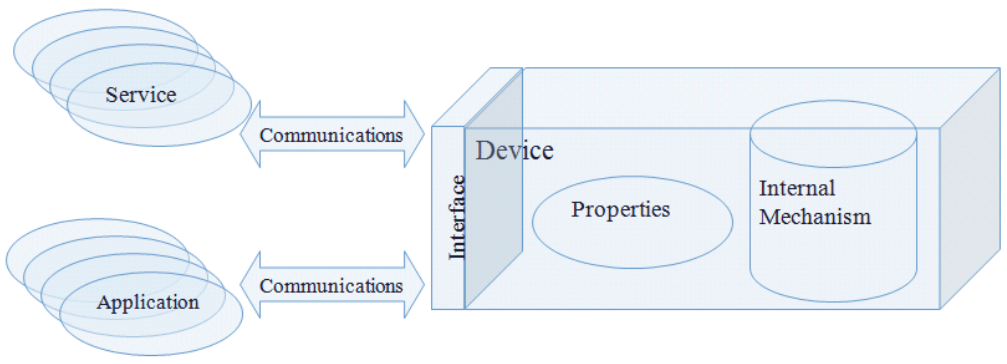
\includegraphics[scale=0.4]{imagens/gatorDDL}
\caption{Caracterização de um dispositivo~\cite{ddlSpec}}
\label{fig:ddlspec}
\end{figure}

Na DDL, um dispositivo é caracterizado como uma entidade com propriedades, mecanismo interno e uma interface, como mostra a Figura~\ref{fig:ddlspec}. As propriedades provêem informações a respeito do dispositivo como seu propósito, suas capacidades, seu fabricante e seus requisitos operacionais. Essas informações são críticas para a integração do sistema e para programadores de serviços. O mecanismo interno é responsável pela operação do dispositivo e é desconhecido do mundo externo. A interface do dispositivo é a ponte entre o hiato do mecanismo interno e do mundo externo. Ela especifica a entrada e saída do dispositivo e provê um guia para aplicações e outros serviços interagirem com o aparelho. A classificação possui flexibilidade para ser extendida e a partir de então estabelecer uma relação hierárquica entre os dispositivos.

Os dispositivos estão classificados em três categorias:
\begin{itemize}
	\item Sensor: apenas provê dados de entrada para o usuário externo.
	\item Atuador: apenas aceita dados de saída do usuário externo.
	\item Dispositivo complexo: provê dados de entrada e aceita dados de saída do usuário externo.
\end{itemize}

Essa classificação, portanto, se apresenta de forma bastante genérica, pois um dispositivo pode se enquadrar como sensor se limitando a fornecer dados de entrada, como atuador, se limitando a receber dados e tomar ações, ou então será classificado como um dispositivo complexo. Logo a categoria de dispositivo complexo poderá ser utilizada por diferentes tipos de recursos, necessitando conhecer as operações definidas no recurso para, a partir dos seviços providos pelo dispositivo, poder inferir que tipo de recurso é aquele. 

De volta ao exemplo apresentado no início deste capítulo, observa-se que as televisões citadas classificariam-se como dispositivos complexos.
